
\begin{center}
\thispagestyle{empty}


\vspace{.5cm}

%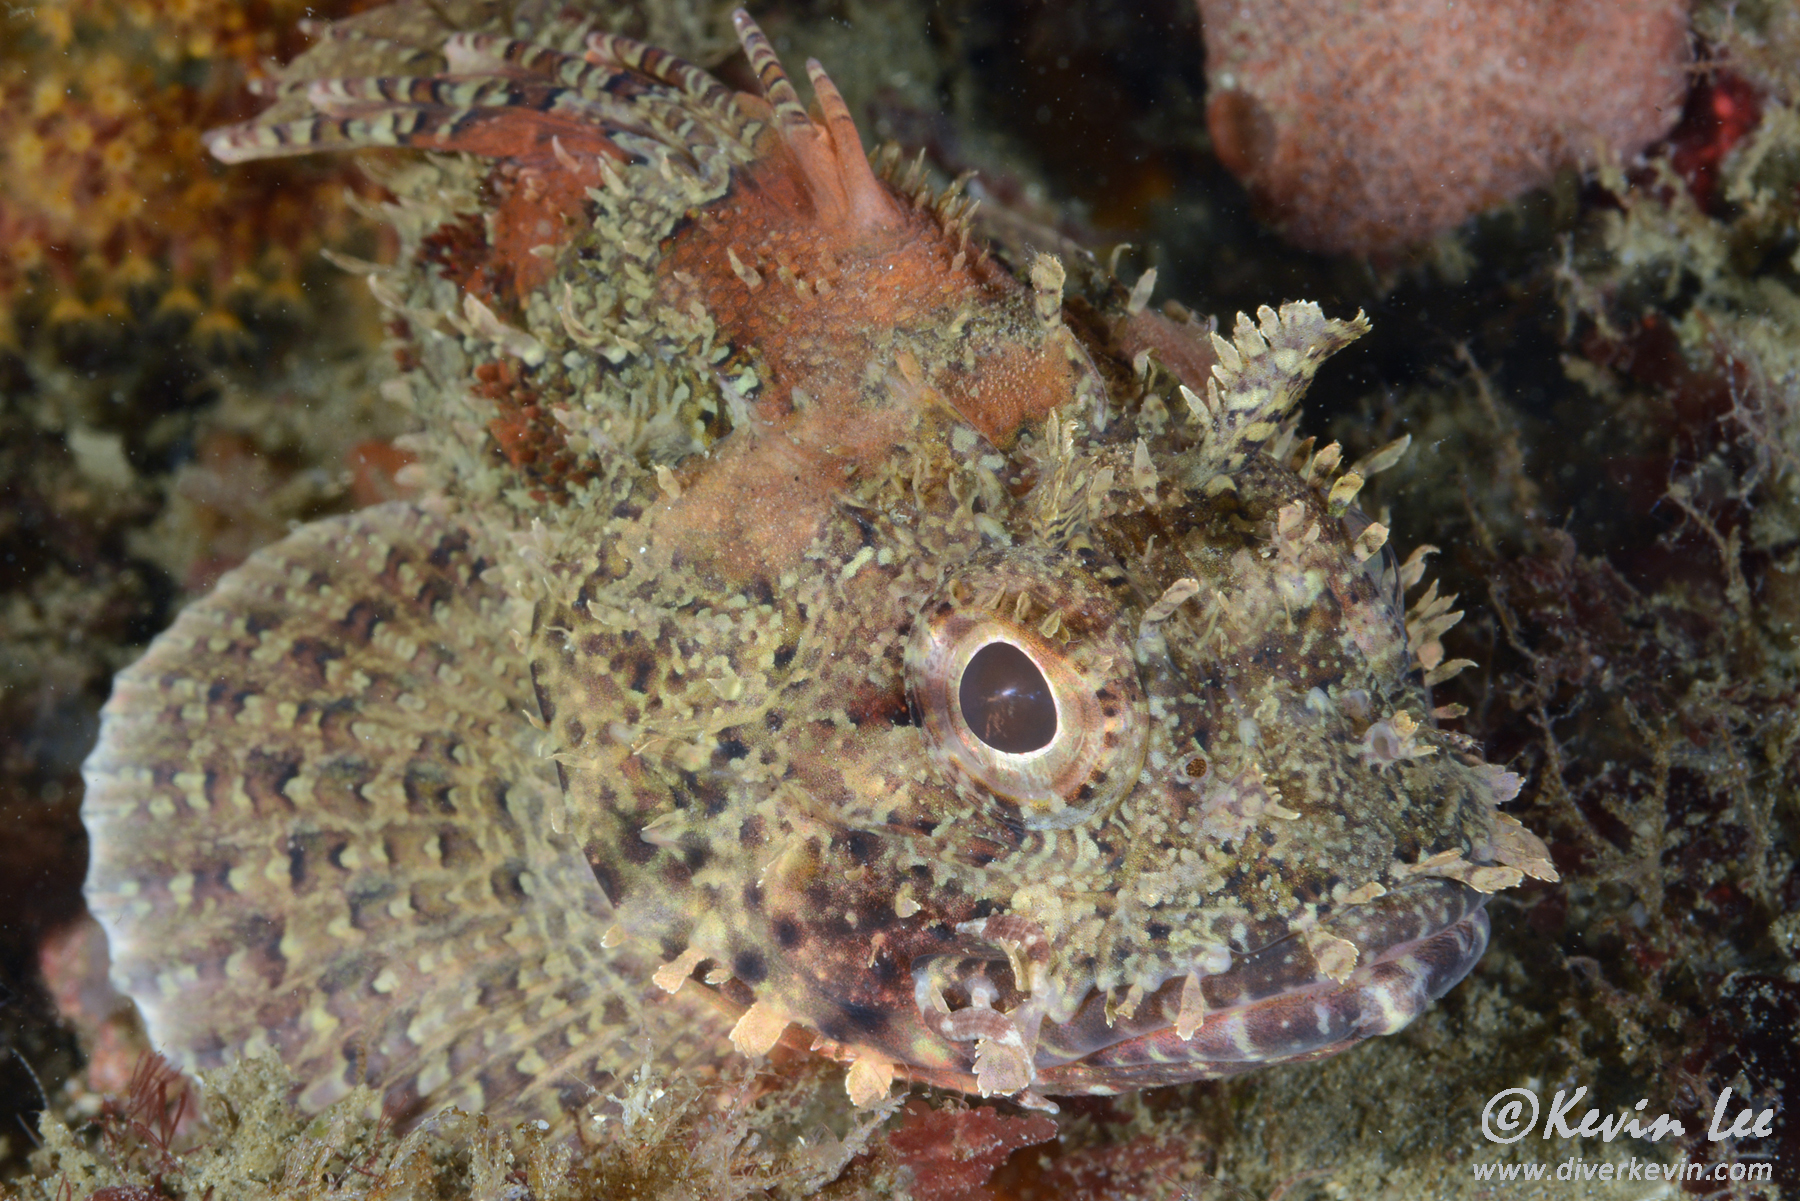
\includegraphics{cover_photo}~\\[1cm]
\pdftooltip{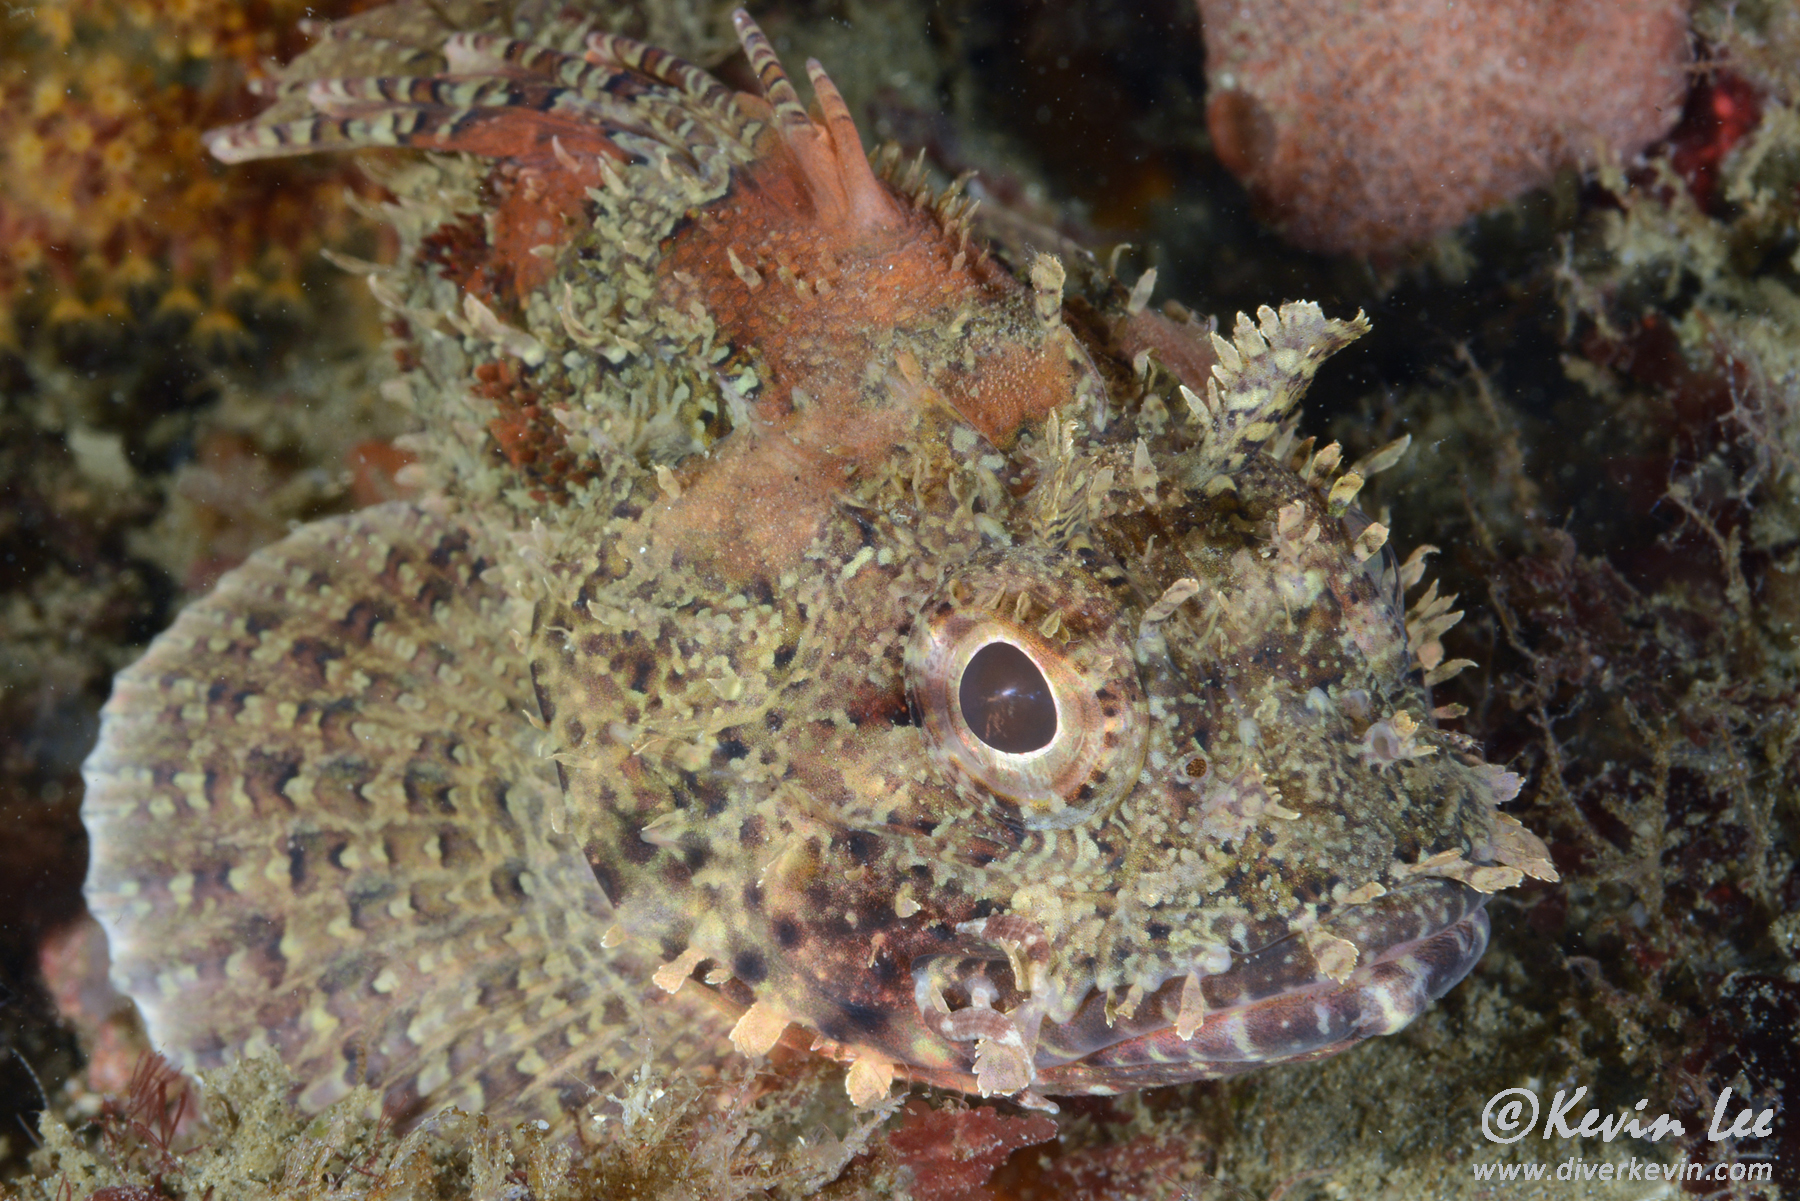
\includegraphics{cover_photo}}{This is a fish.}



Melissa H. Monk\textsuperscript{1}\\
Xi He\textsuperscript{1}\\
John Budrick\textsuperscript{2}\\

\vspace{.5cm}

\small
\textsuperscript{1}Southwest Fisheries Science Center, U.S. Department of Commerce, National Oceanic and Atmospheric Administration, National Marine Fisheries Service, 110 McAllister Road, Santa Cruz, California 95060\\

\vspace{.3cm}

\textsuperscript{2}California Department of Fish and Wildlife, 350 Harbor Blvd., Belmont, California 94002\\


\vspace{.5cm}

\vfill
Disclaimer: This information is distributed solely for the purpose of pre-dissemination
peer review under applicable information quality guidelines. It has not been formally
disseminated by NOAA Fisheries. It does not represent and should not be construed to
represent any agency determination or policy. 

\vspace{.3cm}
%Bottom of the page
%{\large \today}


\newpage

\begin{flushleft}
This report may be cited as:

Monk, M. H. ,He, X., and Budrick, J. 2017. Status of the California Scorpionfish (\emph{Scorpaena guttata}) Off Southern California in 2017. Pacific Fishery Management Council, Portland, OR. Available from http://www.pcouncil.org/groundfish/stock-assessments/
\end{flushleft}

\maketitle

\pagenumbering{roman}
\setcounter{page}{1}
\end{center}


